%% -----------------------------------------------------------------
%% This file uses UTF-8 encoding
%%
%% For compilation use following command:
%% latexmk -pdf -pvc -bibtex thesis
%%
%% -----------------------------------------------------------------
%%                                     _     _      
%%      _ __  _ __ ___  __ _ _ __ ___ | |__ | | ___ 
%%     | '_ \| '__/ _ \/ _` | '_ ` _ \| '_ \| |/ _ \
%%     | |_) | | |  __/ (_| | | | | | | |_) | |  __/
%%     | .__/|_|  \___|\__,_|_| |_| |_|_.__/|_|\___|
%%     |_|                                          
%%
%% -----------------------------------------------------------------

\documentclass{kithesis}

% Additional packages
\usepackage[main=slovak,english]{babel}
% For thesis written in English just change the order of languages:
% \usepackage[main=english,slovak]{babel}

\usepackage{todonotes}
\usepackage{threeparttable}

\usepackage{listings}  % for source code
% Listings settings
% See for details: https://en.wikibooks.org/wiki/LaTeX/Source_Code_Listings
\lstset{
    basicstyle=\small\ttfamily,  % smaller typewriter font
    showstringspaces=false       % don't show spaces in string
}

% Location of file with bibliography resources
\addbibresource{chapters/bibliography.bib}

\newcommand{\detailtexcount}[1]{%
  \immediate\write18{texcount -merge -sum -q #1.tex output.bbl > #1.wcdetail }%
  \verbatiminput{#1.wcdetail}%
}

\newcommand{\quickwordcount}[1]{%
  \immediate\write18{texcount -1 -sum -merge -q #1.tex output.bbl > #1-words.sum }%
  \input{#1-words.sum} words%
}

\newcommand{\quickcharcount}[1]{%
  \immediate\write18{texcount -1 -sum -merge -char -q #1.tex output.bbl > #1-chars.sum }%
  \input{#1-chars.sum} characters (not including spaces)%
}

% Variables
%\thesisspec{figures/thesisspec.png} 

\title{My thesis \br (the skeleton)}{Web crawler pre oblasť internetových správ}

\author{Peter}{Makláry}
\supervisor{Michal Solanik} %veduci prace
%\consultant{Donald E. Knuth} %konzultant
%\college{University of Žilina}{Žilinská univerzita} %univerzita
%\faculty{Faculty of Electrical Engineering and informatics}{Fakulta elektrotechniky a informatiky} %fakulta
%\department{Department of Computers and Informatics}{Katedra počítačov a informatiky} %katedra
%\departmentacr{DCI}{KPI} % skratka katedry
%\thesis{Master thesis}{Diplomová práca} %typ prace
\submissiondate{26}{5}{2023}
%\fieldofstudy{9.2.1 Informatika}
%\studyprogramme{Informatika}
%\city{Košice} %mesto
\keywords{web crawler, data collection, news webs}{web crawler, zber dát, spravodajské weby}
%\declaration{som nepodvadzal}

\abstract{%
    % english 
	This thesis presents the design and implementation of a specialized web crawler for Slovak news websites. Its key advantages include low maintenance and operational requirements, as well as full control over the crawling process. The crawler demonstrates resilience and can operate for extended periods without losing progress in case of failure. Using a modular architecture, the crawler allows easy customization of its behavior. Runtime statistics are collected to monitor the crawling process effectively. In testing, the crawler collected 9 gigabytes of data from 518,000 web pages within 11 hours. 
}{%
    % slovak 
	Táto práca predstavuje návrh a implementáciu špecializovaného webového crawlera pre zber dát zo slovenských spravodajských webov. Jeho hlavnými výhodami je nízka náročnosť na údržbu a prevádzku a plná kontrola nad procesom crawlovania. Crawler preukazuje odolnosť a dokáže dlhodobo fungovať bez straty stavu crawlovania v prípade pádu. Pomocou modulárnej architektúry je možné jednoducho prispôsobiť správanie crawlera. Zbiera štatistiky behu na efektívne monitorovanie crawlovacieho procesu. Počas testovania crawler zozbieral 9 gigabajtov dát z 518 000 webových stránok za 11 hodín. 
}

\thesisspec{figures/zadavaci-list.png}

\acknowledgment{Na tomto mieste by som rád poďakoval svojmu vedúcemu práce za jeho čas a odborné vedenie počas riešenia mojej záverečnej práce.

Rovnako by som sa rád poďakoval svojim rodičom a priateľom za ich podporu a povzbudzovanie počas celého môjho štúdia.
    
V neposlednom rade by som sa rád poďakoval pánom \textit{Donaldovi E. Knuthovi} a \textit{Leslie Lamportovi} za typografický systém \LaTeX, s ktorým som strávil množstvo nezabudnuteľných večerov.}

% if you want to work only on selected chapters
% \includeonly{chapters/analysis} %,chapters/synteza}
% \includeonly{chapters/synthesis} %,chapters/synteza}

% Load acronyms
% Acronyms
% ========
%
% An acronym is a word formed from the initial letters in a phrase. 
%
% Acronym Definition Exapmle:
% ---------------------------
% \newacronym{gcd}{GCD}{Greatest Common Divisor}
% \newacronym{dry}{DRY}{Don't Repeat Yourself}
%
% Usage:
% ------
% You can use these three options:
% 
% \acrlong{}  
%   Displays the phrase which the acronyms stands for. Put the label of the acronym inside the braces. In the example, \acrlong{gcd} prints Greatest Common Divisor. 
%
% \acrshort{} 
%   Prints the acronym whose label is passed as parameter. For instance, \acrshort{gcd} renders as GCD. 
%
% \acrfull{ } 
%   Prints both, the acronym and its definition. In the example the output of \acrfull{dry} is Don't Repeat Yourself (DRY). 
% 
% For more information see:
% -------------------------
% * https://www.sharelatex.com/learn/Glossaries 
% * https://en.wikibooks.org/wiki/LaTeX/Glossary
%


\newacronym{gcd}{GCD}{Greatest Common Divisor}
\newacronym{lcm}{LCM}{Least Common Multiple}



%% -----------------------------------------------------------------
%%          _                                       _   
%%       __| | ___   ___ _   _ _ __ ___   ___ _ __ | |_ 
%%      / _` |/ _ \ / __| | | | '_ ` _ \ / _ \ '_ \| __|
%%     | (_| | (_) | (__| |_| | | | | | |  __/ | | | |_ 
%%      \__,_|\___/ \___|\__,_|_| |_| |_|\___|_| |_|\__|
%%                                                      
%% -----------------------------------------------------------------

\begin{document}
%% Title page, abstract, declaration etc.:
\frontmatter{}

\lstset{language=Scala}

%% List of code listings, if you are using package minted
%\listoflistings

%\pagenumbering{arabic}

%% Chapters
% !TEX root = ../thesis.tex

\chaptermark{Úvod}
\phantomsection
\addcontentsline{toc}{chapter}{Úvod}

\chapter*{Úvod}

S nástupom digitálnej doby sa objem dostupných informácii exponenciálne zväčšuje. Vzniklo množstvo spravodajských webov, publikujúce násobne väčšie množstvo článkov ako ich predchodcovia, printové média. Dokážu sprostredkovať udalosti z celého sveta na minútovej báze. S narastajúcim objemom dát, je za účelom získania vedomostí potrebné efektívne zozbieranie a spracovanie dát. Niekedy to bola úloha knižníc, dnes na to čisto ľudská sila nestačí. Držať krok s digitálnou dobou dokážeme iba ak ju využijeme v náš prospech. Práve program nazývaný web crawler zohráva kľúčovú úlohu pri zbieraní dát zo spravodajských webov. 

Web crawler umožňuje automatizované zbieranie a organizovanie dát zo širokého spektra zdrojov. Minimalizuje potrebu manuálnej práce, čím ušetrí čas a náklady. Spravodajské weby väčšinou neposkytujú zoznam všetkých ich článkov, tie sú rozptýlené a navzájom po-prepájané odkazmi. Crawler umožňuje automatizovane prejsť túto štruktúru a získať o nej informácie. Teda takto vieme zaznamenať aj vzťahy medzi článkami, nie len ich samotný obsah. 

Zbieranie takýchto dát otvára možnosť hĺbkovým analýzam. Z extrahovaných informácii vieme analýzou identifikovať vzorce, trendy a korelácie v spravodajstve. To nám poskytne hodnotný náhľad do mediálneho priestoru. Napríklad hodnotenie vplyvu konkrétnych udalostí, odhaľovanie predsudkov, sledovanie šírenia dezinformácií alebo pochopenie nálad verejnosti voči určitým témam. 

Existuje množstvo dostupných crawlerov. Poväčšine sú ale na účely získania vedomostí z priestoru slovenského spravodajstva príliš robustné a komplexné. Majú vlastnosti, ktoré nepotrebujeme a vyžadujú si priveľké zdroje na prevádzku. Alebo sú jednoduché ale zato málo prispôsobiteľné pre naše potreby. 

Cieľom práce je navrhnutie a implementovanie čo najmenej komplexného crawlera, zbierajúceho dáta zo slovenských spravodajských webov. Musí byť nenáročný na prevádzku a pritom byť nastaviteľný podľa potrieb analýzy. Ako zmena schémy výstupných dát, pridávanie a odoberanie zdrojov. Vlastná implementácia nám dáva možnosť prispôsobiť ho presne pre naše potreby.


% Základom každej analýzy sú kvalitné dáta. Jedným zo zdrojov takýchto dát sú web stránky, kde sú však rozptýlene a uložené v nevhodnej podobe. Tento problém rieši webový crawler.

% Motiváciou práce je príprava dát zo slovenských spravodajských webov na následnú analýzu. Existuje viacero crawlerov, nastaviteľných na získavanie dát pre tieto cieľové účely. Sú ale príliš robustné a vyžadujú si zbytočne veľa zdrojov na prevádzku. 

% Prínosom tejto práce je navrhnutie vlastného riešenia crawlera s modulárnou architektúrou, nízkymi nárokmi na dlhodobú prevádzku a jednoduchým pridávaním zdrojových stránok. Je schopný zotaviť sa po páde a pokračovať kde prestal. Toto riešenie je možné použiť aj pre distribuované crawlovanie, avšak každý výpočtový uzol musí skúmať unikátnu množinu domén. 

% Tento návrh sme implementovali a úspešne pripravili dáta do vhodnej podoby na analýzu v nástroji Apache Spark. 




% Analyzovaním dát nachádzajúcich sa na spravodajských weboch vieme sledovať nálady v spoločnosti, identifikovať stránky šíriace lživé správy alebo skúmať vývoj slovenského jazyka. 

% Na to ale najprv potrebujeme tieto dáta zozbierať a pripraviť do vhodnej podoby. 

% Existuje viacero crawlerov, nastaviteľných na získavanie dát pre tieto cieľové účely. Sú ale príliš robustné a vyžadujú si zbytočne veľa zdrojov na prevádzku. 

% Prínosmi tejto práce

% Navrhnuté riešenie je nenáročné na údržbu, vyžaduje málo zdrojov. Je prispôsobené na dlhodobú prevádzku a odolné voči pádom. 

% Distribuované počítanie sa dá dosiahnuť rozdelením domén a spustením na viacerých počítačoch. 

% tejto práce je navrhnutie vlastného crawlera

% a implementovanie web crawlera prispôsobeného na zbieranie informácii so spravodajských webov.  
% The main contribution of the thesis is the design and implementation of a custom web crawler that is tailored to the needs of news websites. The crawler is designed to be highly configurable and customizable, allowing it to adapt to the specific requirements of different news sources. It is also designed to be efficient and scalable, enabling it to handle large volumes of data without impacting the performance of the target websites.

\chapter*{Formulácia úlohy}

% Text záverečnej práce musí obsahovať sekciu s~formuláciou úlohy resp. úloh riešených v~rámci záverečnej práce. V~tejto časti autor rozvedie spôsob, akým budú riešené úlohy a~tézy formulované v~zadaní práce. Taktiež uvedie prehľad podmienok riešenia.

Cieľom práce je návrh a implementácia crawlera, špecializovaného na zber dát zo slovenských spravodajských webov. Hlavnou podmienkou je, aby dáta boli vhodné na spracovanie nástrojom Apache Spark a dala sa nad nimi spraviť rozumná analýza. Riešenie má byť čo najmenej komplexné a má spĺňať iba zadané požiadavky. Teda nemá mať zbytočné funkcionality, čím by sa zhoršila udržiavateľnosť systému. Závislosť na externých systémoch je dovolená iba v nevyhnutnom prípade. Hlavné požiadavky na systém sú: 

\begin{itemize}
    \item Získavanie dát vhodných na analýzu zo spravodajských webov. Konkrétne: titulok, úvodný paragraf, hlavná časť článku, mená autorov, deň vydania, deň poslednej modifikácie.
    \item Paralelizmus - riešenie musí prechádzať stránky paralelne, ale zároveň nesmie zahlcovať web servery.
    \item Odolnosť voči pádom - ak sa vyskytne chyba, nesmie crawler stratiť dáta.
    \item Redukovanie cieľovej domény - crawler umožnuje nastavovanie filtrovanie stránok na prejdenie.
    \item Pridávanie zdrojov - riešenie musí byť navrhnuté tak aby umožnilo jednoduché pridávanie nových domén na extrakciu. 
    \item Nízka komplexita, jednoduché nasadenie a údržba. 
\end{itemize}


Crawler musí byť schopný pár hodinovej až pár dňovej prevádzky. Teda pri vyhodnotení splnenia cieľov práce musíme preskúmať, či crawler nestráca výkon. Crawler teda musí priebežne zbierať štatistiky o trvaní hlavných operácii. Na ich základe určíme trend a závažnosť prípadnej degradácie. 

Súčasťou práce bude aj demonštratívne použitie zozbieraných dát pre jednoduchú analýzu v nástroji Apache Spark. Tým overíme, že riešenie zbiera dáta ako sme sformulovali v úlohe.
% !TEX root = ../thesis.tex

% \chapter{Analytická časť}

% Analytická časť záverečnej práce analyzuje existujúce podobné prístupy k~riešeniu stanoveného problému. Autor práce musí uviesť v~tejto časti existujúce prístupy a riešenia, pričom musí zaujať stanovisko k~týmto prístupom a riešeniam a opísať ich výhody a nedostatky. Prevažne v~tejto časti autor používa odkazy na použité zdroje. Autor v~analýze nepreberá odseky z~cudzích prác ale uvádza prevažne vlastné postoje podložené odkazmi na literatúru. Analytická časť práce by teda nemala byť len povrchným prepisom základných informácií z~Wikipédie alebo zo stránok opisovaných nástrojov. Je potrebné aby bola analýza podporená aj experimentmi ak to umožňuje téma práce (napr. vyskúšam softvér). Vďaka popisu existujúcich riešení autor pochopí problematiku, viac sa nad riešeniami zamyslí, usporiada si ich, zistí ich kladné a záporné vlastnosti, z~čoho potom postupne vyplynie návrh vlastného riešenia v~syntetickej časti. Analytická časť tvorí zvyčajne ¼ jadra práce.

% Analytickú časť je možné rozdeliť na niekoľko kapitol, ktoré budú venované rôznym analyzovaným témam. Názvy kapitol majú zodpovedať tomu, čo je v~kapitole opisované. Napríklad ak v~práci analyzujete súčasný stav v~oblasti medzigalaktických letov, namiesto všeobecného názvu "`Analýza súčasného stavu"' by mal byť použiťý názov analyzovanej témy --- "`Medzigalaktické lety"'.

% % lorem ipsum
% \section{Lorem ipsum}
% \blindtext

% \section{Aliquam eu malesuada urna}
% \blindtext
% \begin{itemize}
%     \item v~knihe \cite{book} autor prezentuje naozaj odvážne myšlienky
%     \item nemenej zaujímavé výsledky publikuje ďalší autor v~článku \cite{article} 
%     \item v~konferenčnom príspevku \cite{conference} sú uvedené tiež zaujímavé veci
%     \item \LaTeX{}\footnote{\url{https://www.latex-project.org/}} je typografický jazyk
% \end{itemize}

% Given a set of numbers, there are elementary methods to compute its \acrlong{gcd}, which is abbreviated \acrshort{gcd}. This process is similar to that used for the \acrfull{lcm}.

% \subsection{Donec vehicula consequat}
% \blindtext

% \begin{figure}[!ht]
%     \centering
%     
\includegraphics[width=.9\textwidth]{figures/tugboat}
%     \caption{\LaTeX{} Friendly Zone \label{o:latex_friendly_zone}}
% \end{figure}

% \subsection{Nullam in mauris consectetur}
% \blindtext

% \begin{lstlisting}[language=C,caption={Program, ktorý pozdraví celý svet}]
% #include <stdio.h>
% int main() {
%     /* Print Hello, World! */
%     printf("Hello, World!\n");
%     return 0;
% }
% \end{lstlisting}


% \subsection{Vestibulum tristique elementum varius}
% \blindtext

% \begin{table}[!ht]
% 	\caption{Country list}\label{t:1}
% 	\smallskip
% 	\centering

% 	\begin{tabular}{ |p{3cm}||p{3cm}|p{3cm}|p{3cm}|  }
% 		\hline
% 		\multicolumn{4}{|c|}{Country List} \\
% 		\hline
% 		Country Name or Area Name& ISO ALPHA 2 Code &ISO ALPHA 3 Code&ISO numeric Code\\
% 		\hline
% 		Afghanistan & AF & AFG & 004\\
% 		Aland Islands & AX & ALA & 248\\
% 		Albania & AL & ALB & 008\\
% 		Algeria & DZ & DZA & 012\\
% 		American Samoa & AS & ASM & 016\\
% 		Andorra & AD & AND & 020\\
% 		Angola & AO & AGO & 024\\
% 		\hline
% 	\end{tabular}
% \end{table}


% \section{Phasellus id pretium neque}
% \blindtext

% \blindtext

\chapter{Analýza}
\section{Analýza všeobecného Web Crawlera}

Web Crawler, tiež nazývaný ako Spider, je webový bot, ktorý na základe jedného alebo viacerých východiskových URL adries stiahne webové stránky s nimi spojené. Extrahuje hyperlinky obsiahnuté na týchto stránkach a následne pokračuje rekurzívne v sťahovaní webových stránok identifikovanými týmito hyperlinkami. Okrem toho tiež zaznamenáva štruktúru prepojení medzi stránkami. \cite{introToInfRetrieval}

Ich implementácia predstavuje významné inžinierske výzvy v dôsledku rozsahu internetu. Na to, aby prešli podstatnú časť "povrchového webu" v primeranej dobe, musia Web Crawleri sťahovať tisíce stránok za sekundu a zvyčajne sú distribuované na desiatky alebo stovky počítačov. Ich dve hlavné dátové štruktúry - fronta sada URL adries, ktoré ešte neboli prehliadané, a sada objavených URL adries - zvyčajne nevojdú do hlavnej pamäte, takže je potrebné používať efektívne reprezentácie na disku. \cite{encykOfDatabases}

\subsection{Základný algoritmus crawlovania}\label{sub:zakladnyAlgoritmusCrawlovania}
Najjednoduchší algoritmus je sekvenčný, slúži ako základ pre zložitejšie algoritmy využívajúce paralelizmus. 

Algoritmus začína pridaním štartovacích URL adries do fronty. Po jednej sťahuje webové stránky priradené k týmto adresám. Extrahuje z nich URL adresy. Tie pridáva do fronty a stiahnuté stránky ukladá do repozitára.

Tento proces končí vyprázdnením fronty. To v praxi nemusí nastať pretože typické použitia web crawlera si vyžadujú neustále obnovovanie extrahovaných informácii.

\begin{figure}[!ht]
    \centering
    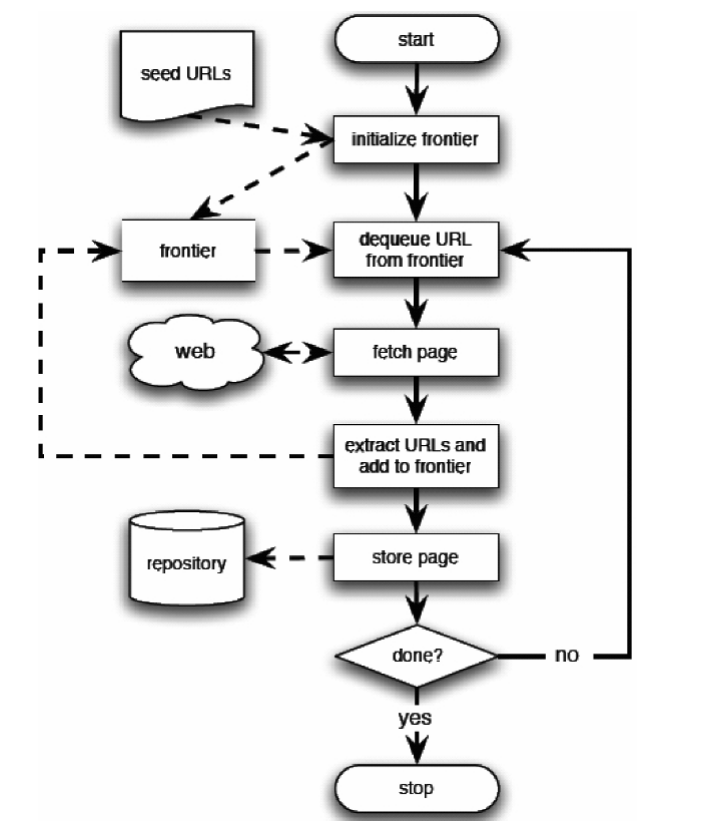
\includegraphics[width=.9\textwidth]{figures/basicCrawlAlgorithm.png}
    \caption{Diagram naivného algoritmu \label{o:basic_crawl_algorithm} \cite{dataMining}}
\end{figure}

\subsection{Fronta} \todo{Premenovat nadpis}
Fronta je centrálny prvok crawlera. Jej implementácia a nastavovanie odráža hlavné vlastnosti systému. 

Naivná implementácia požaduje FIFO dátovú štuktúru s deduplikovaním. Napríklad uchovanie navštívených adries. Pre malé, napríklad POC riešenia je to dostačujúce. 
Všeobecný crawler určený na široký web je typicky distribuovaný a potrebuje stránky znovu navštevovať pre zaručenie aktuálnosti zozbieraných informácii. Taktiež nemá dostatočné zdroje na pokrytie celej domény a musí selektovať adresy na navštívenie. Preto nepostačuje naivné riešenie, a fronta pre praktické využitie musí riešiť tieto požiadavky. 

\subsection{Extractor}
Extraktor je dôležitou súčasťou crawlera, ktorého zodpovednosťou je získavanie URL adries a relevantných údajov zo statických, dynamických webových stránok ale aj obsahu dostupného až po interakcii s vyrenderovanou stránkou (napríkad kliknutie na tlačidlo alebo odoslanie formulára). Teda nemusí ísť len o obyčajný HTML parser. 

Jedna z pozorovaných vlastností extraktora je úspešnosť extrakcie, teda koľko relevantných dát sa podarilo extrahovať z jednej stránky. Môžeme sledovať priemerné úspešnosť naprieč celou prehľadávanou doménou.  

V prípade, že zbierame malé množstvo dát, ktoré sa nachádzajú na väčšine stránkach a majú rovnaký formát, ako napríklad meno autora alebo voľný text, môžeme použiť všeobecný extraktor.  

Doménovo špecifický extraktor je vhodný pre komplexné webové stránky, kde sú údaje netypicky štruktúrované alebo úspešnosť všeobecného extraktora, nie je dostačujúca. 

Po čakaní na odpoveď z web servera ide o druhú časovo najnáročnejšiu časť crawlovania. Preto je nie len úspešnosť ale aj efektivita extraktora dôležitá vlastnosť, hodná pozornosti pri dizajnovaní a optimalizovaní web crawlera.

\subsection{Politiky prehľadávania}
\textbf{Politika výberu} (selection policy) - určuje výber stránok podľa ich relevantnosti, popularite, aktuálnosti a kvalite. Taktiež pomocou nej vieme zúžiť prehľadávanú doménu, ak našim cieľom nie je celý web (napríklad iba e-shopy). Nikto nemá zdroje na prejdenie každej verejne dostupnej stránky, musí sa teda vybrať podmnožina s čo najrelevantnejšími informáciami. Preto je politika výberu kľúčová pre efektivitu crawlera. 

\textbf{Politika znovu navštívenia} (re-visit policy) - určuje ako často môže byť stránka znovu navštívená s cieľom získania aktuálnych informácii. Vo všeobecnosti platí, že čím vyššia frekvencia tým je menšia prehľadávaná podmnožina. 

\textbf{Politika zdvorilosti} (Politeness policy) - stránka si môže určiť, maximum a frekvenciu simultánnych requestov, taktiež sekciu stránok neprístupné pre botov. A to v súbore robots.txt \cite{robotsTxt}. 

\textbf{Politika paralelizácie} (Parallelization policy) - určuje, ako crawler rozdeľuje prácu a koordinuje súbežné prehľadávanie stránok. 

Politiky môžu byť statické - nastavenie pre jednotlivé stránky alebo skupiny stránok na základe ich domény. Napríklad zoznam stránok, ktorým dôverujeme a sú pre nás najpodstatnejšie. \todo{dobry nazov - napriklad index.sme.sk sme je domena}
Alebo dynamické - meniace sa podľa informácii získaných prehľadávaním. Napríklad analýzou obsahu stránky určíme relevantnosť stránok v tej istej doméne. 


\subsection{Vhodné vlastnosti všeobecného crawlera}

\textbf{Odolnosť} - voči pasciam proti botom alebo zle nadizajnovaným stránkam. Napríklad stránky generujúce nekonečnú množinu pod stránok, môžu zahltiť naivný crawler. 

\textbf{Škálovateľnosť} (scalability) - webový priestor sa rýchlo zväčšuje. Aby sa udržal podiel preskúmaných stránok, systém sa musí 
vedieť prispôsobiť. 

\textbf{Distribuovanosť} -  moderný web je mohutný a rýchlo sa meniaci. Pre získanie aktuálneho obrazu, potrebujeme obrovské množstvo dotazov za sekundu, čo vyžaduje distribuovaný systém. 

\textbf{Výkon a efektívnosť} - beh crawlera aj na obmedzenej doméne, vyžaduje robustný systém. Bez dôrazu na efektívnosť sa nám s obmedzenými prostriedkami nepodarí udržať požadovaný pomer spracovaných stránok z celej domény.

\textbf{Prioritizácia} - aplikovanie politiky výberu.

\textbf{Aktuálnosť} - aplikovanie politiky znovu navštívenia.

\textbf{Rozšíriteľnosť} - systém potrebuje spracovávať nové dátové formáty a protokoly. Architektúra by preto mala byť modulárna. 

\textbf{Etickosť} - systém by mal rešpektovať pravidlá v robots.txt.

\section{Použitie Web Crawlera}

\subsection{Použitie v komerčnej sfére}
Web Crawleri sú dôležitou súčasťou internetových vyhľadávačov, kde slúžia na zozbieranie korpusu webových stránok indexovaných vyhľadávačom. Pri čom nie je dôležitý iba obsah stránok ale aj vzťahy medzi nimi. Okrem toho sa používajú v mnohých ďalších aplikáciách, ktoré spracovávajú veľké množstvá webových stránok, ako sú ťažby dát z webov, porovnávacie nákupné enginy \footnote{ napríklad \url{https://www.heureka.sk/}} (comparison shopping engines). \cite{encykOfDatabases}.  

Taktiež na analýzu konkurencie pre dynamické určovanie ceny produktov. Napríklad úprava ceny na základe obsadenosti vstupných lístkov u resalarov (aero-linky). 
Môžu byť použité tiež na monitorovanie zmien a automatickú údržbu web-stránok. A to napríklad identifikovaním nefunkčných adries, kontrola generovanáho obsahu, nedosiahnuteľných assetov a monitorovanie výkonu stránky. \cite{crawlPageTesting}

\subsection{Použitie vo výskume}
Crawler je vhodným nástrojom na získavanie dát pre výskumné účely. Pomocou neho môžu vedci zbierať veľké množstvá dát. Tie môžu neskôr analyzovať a použiť na svoje výskumné účely. Crawler dokáže tieto dáta získať rýchlo a efektívne, čo umožňuje výskumníkom analyzovať trendy a vzory a vytvárať závery na základe veľkého množstva dát. Pre ilustráciu vymenujeme zopár praktických využití dát zozbieraných web crawlerom pre účely výskumu. 

\textbf{Analýza sociálnych sieti a médii} ako Instagram, Facebook, Twitter, Reddit, Youtube a pod. Obsahy príspevok, komentárov, reakcie užívateľov, dokonca aj multimédia ako fotky a videá sú zaujímavé dáta potrebné pre sledovanie nálad a trendov v spoločnosti. Na prípravu datasetov na tieto účely je vhodný crawler zameraný na konkrétne web stránky, v tomto prípade stránky sociálnych médii. Napríklad projekt SocialNetCrawler zbiera dáta na analýzu radikalizácie a extremizácie populácie \cite{socialNetCrawler}.

\textbf{Jazykovedné} skúmanie vývoja jazyka v 21. storočí vyžaduje texty nie len z tlačených médii ale aj z online zdrojov. Crawler vie zozbierať texty a užitočné metadáta z verejných stránok v skúmanom jazyku a to filtrovaním podľa domény najvyššej úrovne (top level domain name) napríklad adresy končiace na .sk.

\textbf{Umelá inteligencia} potrebuje byť natrénovaná na obrovských datasetoch. Práve na ich prípravu sa môže použiť crawler. Napríklad zozbieranie otázok a odpovedí zo stránky Stack Overflow, za účelom vytrénovania AI chat bota. \cite{stackOverflowCrawl}

\subsection{Použitie v oblasti spravodajských webov}
Typickým príkladom sú \textbf{portály zdieľajúce články} z rôznych spravodajských webov. Napríklad služba Google news\footnote{https://news.google.com/}. Táto a jej podobné služby prehľadávajú spravodajské weby a odporúčajú články používateľovi na základe jeho čitateľskej histórie a tém záujmu. Ak článok nie je kategorizovaný, využíva sa NLP (Natural language processing) na extrahovanie tém článkov (topic extraction/classification). Takto sa vedia obohatiť články o ďalšie informácie nevyskytujúce sa priamo na pozorovanej stránke.

\textbf{Agregácia správ v reálnom čase}, pri ktorej je potrebné za čo najkratší čas zozbierať a užívateľovi zobraziť informácie z vybranej skupiny stránok. Napríklad prehľad športových výsledkov. 

Crawlovanie sa taktiež používa pri \textbf{identifikácii nekvalitných článkov} - falošné správy a hoaxy \cite{fakeNews}. Okrem textov sa skúma aj zdrojovanie a prepojenia medzi stránkami. Toto použitie demonštruje dôležitosť získavania nie len obsahu stránok ale aj vzťahov medzi nimi, tie crawler dokáže spracovať do vhodnej formy pre analýzu. Napríklad do grafovej databázy. 



\section{Porovnanie existujúcich riešení} \todo{asi premenovat}
Na trhu je mnoho crawlerov, pohybujúcich sa od SaaS riešení až po nízko úrovňové knižnice. Nie je možné v tejto práci porovnať všetky z nich. Vybrali sme tri open-source projekty ako zástupcov, s rôznymi prístupmi, zameraniami a zložitosťou použitia.

\subsection{News-please}
News-please\footnote{https://github.com/fhamborg/news-please} je open-source crawler zameraný na extrahovanie názvu článku, úvodného paragrafu, hlavného textu, hlavného obrázka, mien autorov, dňa vydania a jazyka článku. Je spustiteľný po malých modifikáciách hneď po inštalácii, nevyžaduje si zasahovanie do kódu. Ovláda sa cez CLI, čo ho robí oproti iným open-source riešeniam vhodným nástrojom pre vedcov a analytikov s obmedzenými alebo žiadnymi programátorskými schopnosťami. Je postavený na Scrapy frameworku. 

Extrahovanie dát z článkov prebieha bez potreby modifikácie, či už kódu, alebo cez CLI. To neplatí pre iné riešenia, tie si vyžadujú implementovanie extraktora alebo jeho nastavenie. Použitý extraktor v crawlery news-please dosahuje úspešnosť 60\% až 80\% \cite{newsPlease}. Čo je dostačujúce pre zbieranie dát zo širokého korpusu spravodajských webov. Napríklad pre analýzu sentimentu v spravodajstve. To ale nemusí dostačovať pre zbieranie dát z úzkeho korpusu, teda z malého počtu domén. 

News-please neposkytuje pohodlné a praktické nastavenia extraktora. Taktiež nie je ľahko modifikovateľný pre špecifické použitie a optimalizovanie. Jeho výhodou je rýchle a jednoduché nasadenie a relatívne vysoko úspešný extraktor. 

Nepodporuje poriadnu distribúciu a horizontálnu škálovateľnosť. Ak budeme nedostatočným výkonom nútení použiť viac výpočetných jednotiek, môžeme rozdeliť prehľadávané stránky podľa doménového mena. Teda každá výpočetná jednotka dostane skupinu doménových mien na prehľadanie. Takéto riešenie nie je ale dostatočne robustné pre všetky aplikácie. 

\subsection{Scrapy} 
Scrapy je Python open-source framework, určený na implementovanie web crawlerow. Oproti News-please ide len o framework pomocou, ktorého sa dá vytvoriť crawler. Nejde teda o samostatnú aplikáciu. 

Jeho API je relatívny vysoko abstraktné, teda používateľ nie je nútený riešiť implementačné detaily. Tvorca crawlera implementuje logiku crawlovania, hlavne extraktor a ukladanie získaných dát.

Je vysoko flexibilný, čo ho robí ale aj náročnejším na použitie. To je vyvážene zdravou a veľkou komunitou. Taktiež aj kvalitnou dokumentáciou. 

Medzi hlavné nevýhody patrí absencia podpory spustenia v distribuovanom systéme. Dá sa to obísť rovnakou mechanikou ako je popísaná pre news-please. Odporúča ju aj oficiálna dokumentácia\footnote{https://docs.scrapy.org/en/latest/topics/practices.html}. Rozdelenie stránok, distribúcia a škálovanie je už na na tvorcovi crawlera. 

\subsection{Apache Nutch}
Apache Nutch je vďaka pluginovej architektúre vysoko rozšíriteľný crawler. Podporuje distribúciu a horizontálnu škálovateľnosť, to ho robí vhodným nástrojom pre vybudovanie vysoko výkonných crawlovacích botov. Schopnosť pridávať a nahradzovať pluginy a rozšírenia umožňuje programátorom modifikovať takmer celé správanie. Môže ísť napríklad o pridanie nového dátového zdroja, zmenu extraktora alebo aj o zmenu logiky paralelizácie. 

Veľkou výhodou kompatibilita s ďalšími Apache Software Foundation projektami ako Hadoop, ZooKeeper, Spark, Hive a ďalšími. To znamené, že Nutch vie jednoducho využiť ich silné stránky, napríklad Hadoop distribuovaný súborový systém alebo možnosti distribuovaného spracovania dát ponúkané Sparkom. Táto kompatibilita uľahčuje použitie Nutch v rozsiahlych aplikáciach ako napríklad budovanie indexu vyhľadávača. 

Avšak, rovnako ako iné vysoko distribuované systémy, nasadenie, konfigurácia a údržba Apache Nutch môže byť komplexná a náročná úloha. Systém vyžaduje značné zdroje vrátane úložného priestoru, pamäte a výpočtového výkonu, čo nemusí byť vhodné pre menšie projekty. Navyše, kvôli zložitosti systému si môže vyžadovať viac technických a programátorských znalostí, ako predchádzajúce riešenia.

% !TEX root = ../thesis.tex

\chapter{Syntetická časť}
\label{methodology}

Syntetická časť opisuje metódy použité na syntézu riešenia a opisuje syntézu samotného riešenia (zvyčajne je to návrh/implementácia softvérového resp. hardvérového riešenia), pričom sa opiera o~závery analytickej časti práce. Začína od toho, ako sa bude riešenie používať: najdôležitejšie scenáre používania a používateľské rozhranie, ktoré bude tieto scenáre efektívne podporovať. Až potom je na rade vnútorná architektúra alebo použité technológie. Syntetická časť tvorí zvyčajne ½ jadra práce.

Syntetickú časť práce vhodne rozdeľte do kapitol a pomenujte ich podľa toho, čomu sú venované.

\chapter{Implementácia}
\label{implementation}

V tejto kapitole podrobne popíšeme implementáciu podla návrhu v predchádzajúcej kapitole. \todo{Dopisat uvod ked bude kapitola hotova}

\begin{figure}[!ht]
    \centering
    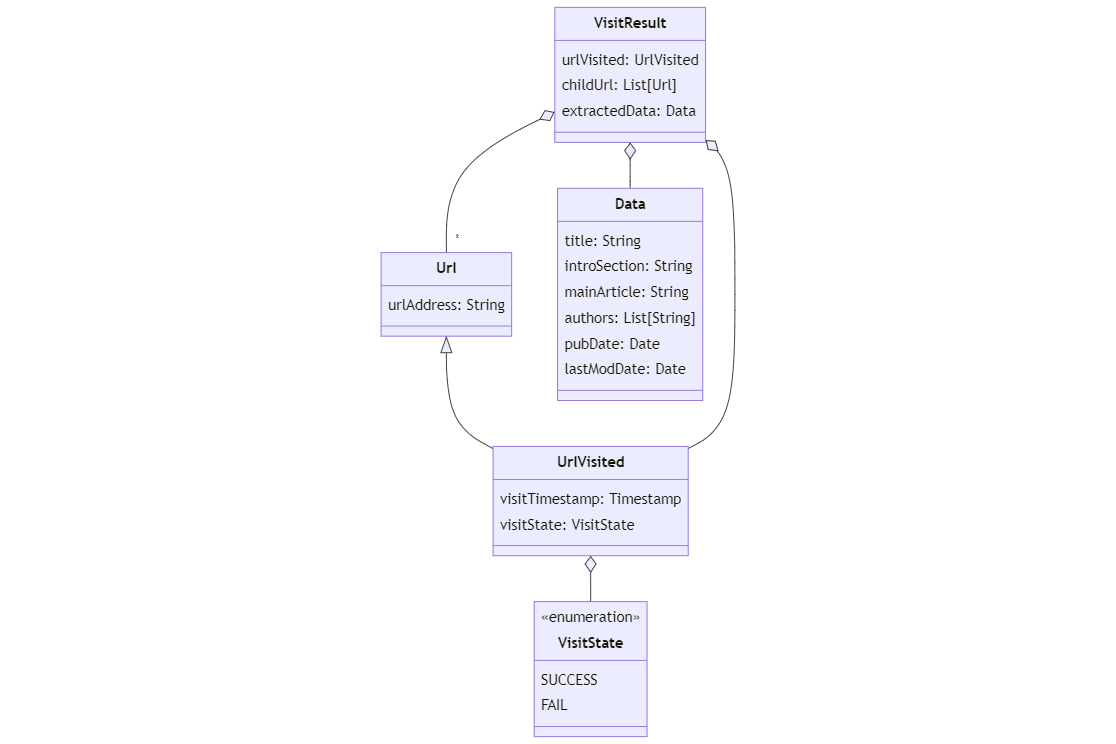
\includegraphics[width=.9\textwidth]{figures/classDiagramVisitResult.png}
    \caption{Class diagram pomocných dátových štruktúr \label{o:classDiagramVisitResult}}
\end{figure}

\section{Implementacia modulov}
V návrhu architektúry sme rozdelili riešenie do 4 základných modulov a popísali ich zodpovednosť a základnú komunikáciu medzi nimi. Taktiež sme popísali prístup k paralelizácii. V tejto podkapitole na to nadviažeme a popíšeme ako sme implementovali tieto moduly. 

\subsection{Orchestrátor}
Tento modul je vlastne jadro aplikácie, integrujúci zvyšné moduly. Tie komunikujú výlučne s ním a nie medzi sebou. Táto separácia nám umožnila jednoduché testovanie jednotlivých modulov a sledovanie komunikácie medzi nimi.

V implementácii sme nepoužili priamo pojem orchestrátor, ale implementovali sme ho v triede Crawler. Tá reprezentuje celú našu aplikáciu a jej metóda \textit{crawlMainJob} \todo{Ako pomenuvavat metody, oznacit ze ide o nazvy z kodu} štartuje samotný crawling. 

Pre jej inicializáciu musíme dodať objekt triedy CrawlerContext, obaľujúci inštancie zvyšných modulov. Takto vieme spúšťať crawler s rôznymi implementáciami modulov a tým meniť jeho správanie. Ide vlastne o známy princíp injektovania závislostí (dependency injection). \todo{Ak treba popisat benefity}

Po spustení sa vykonáva krok crowlovania, implementovaný funkciou doStep. Čo sa vykonáva v kroku je popísané v návrhu. Za zmienku ale stojí, že rozdelenie práce pracovným vláknam a agregovanie výsledku je presunuté do funkcie crawlStep. Tá pre pole adries vráti objekt CrawlResult. Bližšie si jej implementáciu popíšeme v samostatnej podkapitole. 

Návratovou hodnotou doStep je trieda RunStats. Tú priebežne agregujeme do CrawlerRunReport. Ide napríklad o počet navštívených adries a počet nezdarov. Využili sme triedy ako BigInt, kedže rátame s dlhodobým behom. 

\subsection{Funkcia crawlStep}
Táto funkcia rozdelí poskytnuté adresy parametrom do skupín. Každá skupina je potom spracovaná jedným z pracovných vlákien. Počet skupín je v štandardnom nastavení väčší ako počet pracovných vlákien. Tým zvýšime vyrovnanosť záťaže jednotlivých vlákien.

Využili sme abstrakciu nad paralelným spracovaním - \textit{Future}. Ide o generickú triedu štandardnej scala knižnice reprezentujúca budúcu hodnotu. V našom prípade budúcu hodnotu CrawlResult. Z pohľadu funkcionálneho programovanie je to monád. Tento prístup sa stáva populárnym aj v nie plno funkcionálnych programovacích jazykoch ako Java, Python a podobne. 

Práca vlákna je reprezentovaná funkciou crawlChunk. Tá mapuje skupinu adries na budúcu hodnotu CrawlResult. 

Funkcia crawlStep čaká na všetky budúce hodnoty, následne agreguje čiastkové výsledky práce do jedného. Reprezentujúceho výsledok navštívenia a extrahovania stránok určených na spracovanie v tomto kroku. 

Teda všetká paralelná činnosť programu je izolovaná v tejto funkcii. 

\subsection{Repozitár}
Modul repozitár reprezentuje interface s jednou metódou - saveStep. Jej jediný parameter je pole objektov RepoDTO (Data Transfer Objekt). Tento objekt reprezentuje schému ukladaných dát a je nezávislý na reprezentácií týchto dát vo zvyšku programu - PageResult. 

Táto striktná nezávislosť nám umožní v budúcnosti zmeniť spôsob ukladania výsledkov napríklad do relačnej databázy bez zásahu do zvyšku programu. Vytvoríme iba novú implementáciu tohto interfacu a vložíme ju do objektu CrawlerContext. 

Vytvorili sme 2 základné implementácie a jednú určenú na testovanie. Prvá ukladá výsledky všetkých krokov do jedného CSV súboru. To je vhodné pre krátke behy hlavne pri optimalizácii parametrov. Druhá ukladá každý krok do samostatného CSV. Pre produkčné nasadenie používame druhú implementáciu. 

Implementácia určená na testovanie ukladá objekty RepoDTO iba do vnútorného poľa. A pridáva metódu getAllSaved. To využívame v integračných testoch. Takto vieme skontrolovať či sa ukladajú do repozitára požadované výsledky a nemusíme pozerať do súborového systému. 


\subsection{Url Manažér}
Tento modul je reprezentovaný interfacom s metódami:
\begin{itemize}
    \item Upsert pridá Url adresy na prejdenie v budúcich krokoch. 
    \item GetBatch vráti adresy na prejdenie v aktuálnom kroku. 
    \item markAsCrawled označí adresy ako prejdené
\end{itemize}


Pri návrhu sme sa obávali, že nám uchovanie v operačnej pamäti nebude stačiť a budeme nútený použiť databázu. Ale testovanie aplikácie nepotvrdili túto obavu. Teda pre zníženie náročnosti na údržbu a infraštruktúru sme sa rozhodli pre jednoduchšie riešenie.

Hlavná implementácia tohto modulu ukladá potrebné dáta v operačnej pamäti a po každom volaní metód upsert a markAsCrawled je serializovaná na disk. Ako sme spomínali v návrhovej časti práce, zodpovednosťou tohto modulu je uchovanie stavu aj napriek pádom. 


Riešenie je pripravené na rozšírenie. V prípade potreby stačí implementovať tento modul robustnejšie a vložiť ho do CrawlerContext. 

\subsection{Extraktor}
Extraktor je implementovaný funkciou crawlUrl. Tá využíva interface DomainScraper s metódami na extrahovanie dát z html  dokumentu (parseDocument) a rozhodnutia či adresa je v danej doméne. Výsledkom extrahovania dát zo stránky je objekt PageContent. 

Následne funkcia crawlUrl odfiltruje podporované dcérske adresy pomocou triedy DomainFilter. Tie spolu s ďalšími hodnotami vráti v objekte CrawlResult. 

Crawled obsahuje teda iba pole podporovaných adries. PageContent na druhú stranu obsahuje všetky adresy nájdené na stránke. 

Pre pridanie podpory extrahovania z novej domény je potrebné implementovať DomainScraper a túto implementáciu pridať do zoznamu podporovaných domén. 


\section{Využitie parciálnej aplikácie funkcií vyššieho rádu}
Parciálna aplikácia je technika funkcionálneho programovania na zvýšenie znovu použiteľnosti funkcií, čitateľnosti a v našom prípade hlavne injektovania závislostí. Funkcia vyššieho rádu je funkcia berúca inú funkciu ako parameter alebo ako návratovú hodnotu. 

My sme tieto techniky využili hlavne pre injektovanie extraktora. Tento modul sme implementovali ako funkciu crawlUrl. Tá mapuje url na CrawlResult. Potrebuje získať html zo servera a extrahovať z neho relevantné dáta. 

Pre neprodukčné účely ako napríklad testovanie je pripájanie na server nežiadúce a chceme deterministickú implementáciu tejto funkcie. Tú vieme podsunúť ako parameter funkcii vyššieho rádu crawlChunk a crawlStep. Bližšie to popíšeme v podkapitole o testovní crawlera. 

\section{Zastavenie crawlera}
Za zastavenie crawlera mimo vyčerpania prehľadávanej fronty je zodpovedný interface CrawlLimit s metódou: shouldStopCrawling. Imeplementáciu poskytneme crawleru pri jeho inicializácii, takto vieme meniť podmienky zastavenia bez zásahu do kódu crawlera. Vytvorili sme 3 implementácie: 

\begin{itemize}
    \item StepLimitedCrawl - limitujeme počtom krokov.
    \item TimeLimitedCrawl - limitujeme ubehnutým časom od inicializácie, zastavíme crawlovanie až po skončení posledného kroku. 
    \item InfiniteCrawl - crawlovanie bez limitu.
\end{itemize}


\section{Testovanie}
Vďaka vhodnej architektúre môžeme každý modul mimo orchestrátora otestovať zvlášť. A orchestrátor otestovať spomínaným injektovaním závislostí. Takto poskytneme testovacie implementácie modulov pre izolované testovanie správania  orchestrátora. Využívame jednotkové testy (unit tests). 

Integračnými testami testujeme hlavný scenár krolovania, teda či všetky moduly spolu komunikujú korektne. 

Beh crawlera je riadený odpoveďami zo serverov. Pre testovanie teda musíme nahradiť tieto odpovede. Posunuli sme to kúsok ďalej a nahrádzame celý extractor. Teda priradenie CrawlResult zadanej adrese. Práve na to sme využili spomínané parciálne aplikovanie funkcii vyššieho rádu.

Takto vieme vytvárať testovacie scenáre jednoducho, rýchlo a bez potreby písania html súborov. Stačí nám pre každý test vytvoriť funkciu priraďujúcu CrawlResult zadanej adrese. Príklad takejto funkcie uvádzame nižšie. Týmto spôsobom otestujeme takmer celú aplikáciu.

\begin{lstlisting}
    (u: Url) => u match {
        case "aaaa" => CrawlResult().addCrawled(crawled1)
        case "bbbb" => CrawlResult().addCrawled(crawled2)
        case "xxx" => CrawlResult().addFailed(Failed(u, "Url not supported"))
      }
\end{lstlisting}


Extraktor testujeme zvlášť na zopár pripravených HTML súboroch. Taktiež zopár testov sa priamo pripája na servery. Je ich malý počet a vieme ich spúšťať samostatne od hlavných testov. Teda zredukovali sme nezávislosť testov na minimum. 

\section{Logovanie}
Veľkú pozornosť sme kládli na dôkladné logovanie. Rátame s niekoľkohodinovým až pár dňovým behom aplikácie. V prípade pádu programu alebo nájdenia chyby potrebujeme čo najviac informácii o tomto behu.

Využili sme java knižnicu na logovanie ale obalili sme ju našou knižnicou. Pridali sme meranie času od posledného zápisu. Taktiež pohodlné meranie a zápis času behu častí programu. To sme využili pri odhaľovaní miest degradácie výkonu pri dlhých behoch. V príklade nižšie môžeme vidieť použitie pri meraní dĺžky získavania adries na prejdenie v kroku. 

\begin{lstlisting}
    te("Getting Batch"){ctx.urlManager.getBatch(stepMaxSize)}
\end{lstlisting}

Výstup v zázneme vyzerá takto:  "Getting Batch -- Start,
    Getting Batch -- End | Time delta from last timed log (millis): 5 | Now: 2023-05-10T16:20:52.557005500"



\section{Výzvy ktorým sme čelili pri implementácii riešenia}
Prvá implementácia využívala polymorfizmus pre rozdielne správanie tried Crawled a Failed. Napríklad pri zápise do repozitára, alebo pri agregovaní štatistík. 

To ale spravilo tieto triedy zodpovednými za veľkú časť funkcionality crawlera. Od interakcie s repozitárom po ukladanie adries na nasledujúce prechádzanie. Čo je samozrejme zlý dizajn. 

Preto sme sa rozhodli prerobiť aplikáciu a využiť kompozíciu na miesto dedičnosti. Čo nám umožnilo lepšie oddelenie zodpovedností. 
% !TEX root = ../thesis.tex

\chapter{Vyhodnotenie}
\label{evaluation}

Vyhodnocovacia časť je kľúčovou časťou záverečnej práce. Tato časť obsahuje vyhodnotenie navrhnutého (vytvoreného) riešenia. Uprednostňované je objektívne vyhodnotenie výsledkov práce, ktoré sa opiera o~meranie a štatistické metódy, prípadne matematické dôkazy. V~prípade nameraných hodnôt musí autor opísať metódu merania, priebeh merania, výsledky a interpretáciu výsledkov v~kontexte riešeného problému a stanovených cieľov. Na základe vyhodnotenia riešenia autor opíše prínosy svojej práce. Vyhodnocovacia časť tvorí zvyčajne ¼ jadra práce.

% !TEX root = ../thesis.tex

\chapter{Záver}
\label{summary}

% Záver práce obsahuje zhrnutie výsledkov práce s~jasným opisom prínosov a pôvodných (vlastných) výsledkov autora a vyhodnotenie splnenia stanovených cieľov. Je to stručné zhrnutie informácií uvedených v~záverečnej práci. Záver by nemal obsahovať nové informácie.

% V~závere by mal tiež autor poukázať na prípadné otvorené otázky, ktoré sú nad rámec rozsahu práce a mal by odporučiť ďalšie aktivity na pokračovanie pri riešení problému. Rozsah záveru je minimálne 1 celá strana.

V tejto práci sme navrhli a implementovali crawler špecializovaný na zber dát zo slovenských spravodajských webov. Jeho veľkou výhodou oproti použitiu existujúcich riešení je nenáročnosť na údržbu a prevádzku a plná kontrola nad priebehom crawlovania. Je schopný dlhodobej prevádzky a je odolný voči pádom. Ak sa vyskytne chyba, vieme proces opätovne spustiť bez straty stavu crowlovania. 

Architektúru sme zvolili modulárnu čím sme umožnili jednoduchú úpravu správania. Napríklad ak sa v budúcnosti rozhodneme ukladať dáta do iného formátu, implementujeme modul zodpovedný za ukladanie výsledkov a poskytneme jeho inštanciu crawleru pomocou injektovania závislostí.  

Paralelizmus sme izolovali od ostatných modulov. Tie teda nemajú žiadnu paralelizačnú logiku. Vďaka tomu, je údržba nenáročná. 

Program zbiera štatistiky o behu ako napríklad trvanie najdôležitejších operácii a úspešnosť extrakcie dát. Pomocou nich vieme monitorovať nasadené crawlery. 

Vytvoreným riešením sme za 11 hodín zozbierali 9 gigabajtov dát z 518 000 web stránok. Na týchto dátach sme v nástroji Apache Spark vykonali jednoduchú analýzu spätných odkazov. Čím sme identifikovali aktuálne odporúčané články a články s najväčším dosahom. Týmto sme overili splnenie hlavného cieľa práce a to schopnosť zozbierať dáta na podobné účely.  

Zo zozbieraných štatistík sme vyhodnotili, že naše riešenie je vhodné na behy trvajúce hodiny. Avšak po pár dňoch degraduje výkon na nežiadúcu úroveň. Je to z dôvodu ukladania prejdených adries v pamäti a ich perzistovanie na disk v každom kroku. V tomto ohľade navrhujeme pre budúce prácu upraviť perzistovanie z kompletnej serializácie v každom kroku, na perzistovanie iba inkrementov. 

Pri analýze štatistík z behu sme pozorovali prerušenie poklesu adries náhlym prudkým nárastom. V kapitole \ref{c:addInteresting} sa mu povrchovo venujeme. Považujeme ho za zaujímavý úkaz hodný hlbšieho preskúmania v inej práci.  


% good linebraking of bibtex url
\setcounter{biburllcpenalty}{7000}
\setcounter{biburlucpenalty}{8000}

%% The bibliography
\printbibliography[heading=bibintoc]

\label{theend} % the last page of the thesis

% List of acronyms
\printglossary[type=\acronymtype,title={\acrlistname}]

% Glossaries
\printglossary

%% Appendix
% !TEX root = ../thesis.tex

\chapter*{\appendixlistname}
\addcontentsline{toc}{chapter}{\appendixlistname}

\begin{description}
	\item[\appendixname{} A] Používateľská príručka
    \item[\appendixname{} A] Systémový manuál
    \item[\appendixname{} C] CD médium -- záverečná práca v~elektronickej podobe,
    % \item[\appendixname{} C] Používateľská príručka
    % \item[\appendixname{} D] Systémová príručka
\end{description}

\appendix
\renewcommand\chaptername{\appendixname}
% !TEX root = ../thesis.tex

\chapter{Používateľská príručka}

% \section*{Karel's Primitives}

% \begin{itemize}
%     \item \verb|void movek()| - Moves \textit{Karel} one intersection forward.
%     \item \verb|void turn_left()| - Pivots \textit{Karel} $90$ degrees left.
%     \item \verb|void pick_beeper()| - Takes a beeper from the current intersection and puts it in the beeper bag.
%     \item \verb|void put_beeper()| - Takes a beeper from the beeper bag and puts it at the current intersection.
%     \item \verb|void turn_on(char* path)| - Turns \textit{Karel} on.
%     \item \verb|void turn_off()| - Turns \textit{Karel} off.
% \end{itemize}


% \section*{Karel's Sensors}

% \begin{itemize}
%     \item \verb|int front_is_clear()| - Returns \texttt{1} if there is no wall directly in front of \textit{Karel}. \texttt{0} if there is.
%     \item \verb|int right_is_clear()| - Returns \texttt{1} if there is no wall immediately to \textit{Karel}'s right. \texttt{0} if there is.
%     \item \verb|int beepers_present()| - Returns \texttt{1} if \textit{Karel} is standing at an intersection that has a beeper. \texttt{0} otherwise.
%     \item \verb|int facing_north()| - Returns \texttt{1} if \textit{Karel} is facing north. \texttt{0} otherwise.
%     \item \verb|int beepers_in_bag()| - Returns \texttt{1} if there is at least one beeper in \textit{Karel}'s beeper bag. \texttt{0} if the beeper bag is empty.
% \end{itemize}


% \section*{Misc Functions}

% \begin{itemize}
%     \item \verb|void set_step_delay(int)| - Sets delay of one \textit{Karel}'s step in miliseconds.
%     \item \verb|loop(int)| - Repeats \textit{Karel}'s instruction in a loop.
% \end{itemize}


Táto príručka je určená pre správcu crawlera. Rozoberieme si ako crawler inicializovať a monitorovať jeho beh.

\section{Príprava prostredia}
Crawler nie je závislí na žiadnom externom systéme. Teda netreba nasadzovať databázu ani nič podobné. 

Je potrebné mať JRE (Java Runtime Environment), ale odporúčame JDK (Java Development Kit) verzie 11. 

\section{Inicializácia}
Pri inicializácii vieme crawleru poskytnúť rôzne implementácie modulov a tým ovplyvniť jeho správanie. Napríklad ak bude potrebné zmeniť ukladanie výsledkov z CSV formátu do iného, stačí implementovať novú verziu repozitára a pri inicializácii ňou naplniť CrawlerContext. Podrobný postup je znázornený na diagrame \ref{o:initChart}.

Dôležitou súčasťou nastavení je aj veľkosť kroku (stepMaxSize), udávajúca počet adries spracovaných v jednom kroku. Jej zvýšením vieme zefektívniť beh programu, keďže redukujeme počet neparalelných úsekov a prístup do súborového systému. Na druhú stranu ale zvyšujeme nároky na pamäť, keďže v nej pred uložením držíme práve tento počet výsledkov extrahovania. Teda ak zvo-
líme tento parameter príliš vysoký, program môže vyčerpať pridelenú operačnú pamäť. Oproti tomu menším problémom je aj zväčšenie veľkosti stratených dát pri páde programu.

\begin{figure}[!ht]
    \centering
    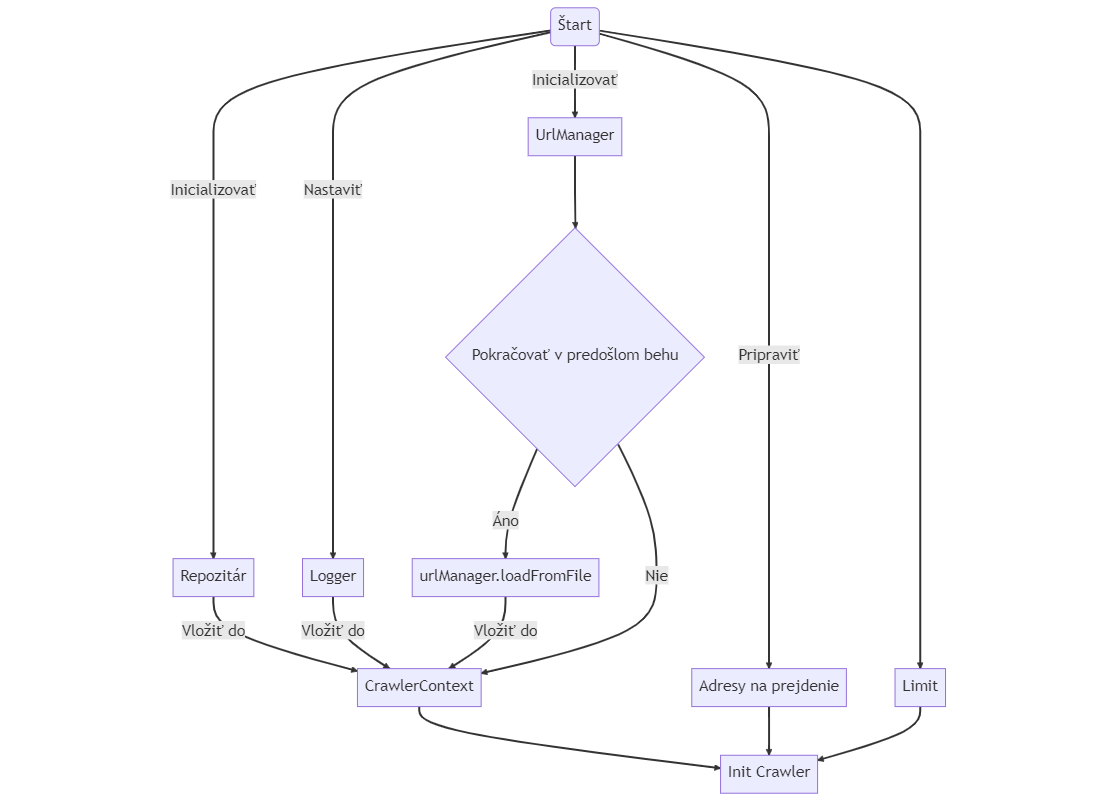
\includegraphics[width=1\textwidth]{figures/initChart.png}
    \caption{Diagram inicializácie crawlera\label{o:initChart}}
\end{figure}

\begin{figure}[!ht]
    \centering
    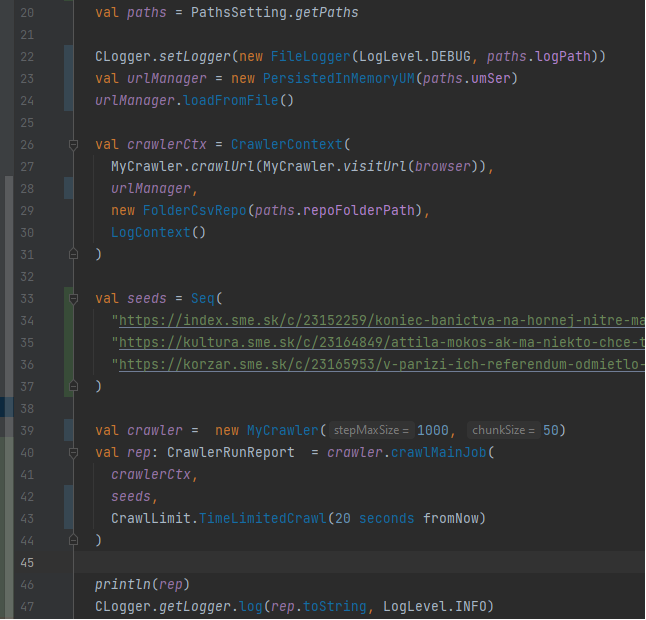
\includegraphics[width=.9\textwidth]{figures/crawlInit.png}
    \caption{Ukážková iniclializácia crawlera\label{o:initCrawl2}}
\end{figure}

\section{Vyhodnotenie štatistík}
Crawler zbiera štatistiky pomocou záznamov ukladaných do súbory. Skript \textit{MakeStatsFromLogs} ich potom spracuje a zapíše do CSV súboru. 

Odporúčame každý jeden stĺpec dať do samostatného grafu. Výsznam stĺpcov: 
\begin{itemize}
    \item \textbf{crawlT} - trvanie crawlovacej aktivity - jej plávajúci priemer má byť konštantný , rastúci trend indikuje problém s pripojením na server pravdepodobne zapríčinenú príliš veľkou paralelizáciou (nanosekundy)
    \item \textbf{stepT} - dĺžka jedného kroku - tiež by mala byť konštantná (milisekundy)
    \item \textbf{batchT} - trvanie získania adries na prejdenie v danom kroku (nanosekundy)
    \item \textbf{upsertT} - trvanie pridania nových adries na prejdenie - očakávame mierny lineárny nárast (nanosekundy)
    \item \textbf{upsertT} - trvanie pridania nových adries na prejdenie - očakávame mierny lineárny nárast (nanosekundy)
\end{itemize}




\chapter{Systémový manuál}

Tento manuál slúži pre popísanie crawlera na úrovni vhodnej pre úpravu systému a rozširovanie jeho funkcionalít. 

% Scala je vysoko úrovňoví jazyk schopný lepšej reprezentácie abstrakcie ako diagramy a bežná ľudská reč. Táto dokumentácie je určená primárne pre programátora so znalosťou tohto jazyka, preto popisuje len zodpovednosti modulov. 

\section{Moduly}
V tejto podkapitole popíšeme stručne zodpovednosť modulov a ich rozhranie voči zvyšku systému. 

\subsection{UrlManager}
Modul zodpovedný za ukladanie stavu crawlovania a jeho perzistovanie. Hlavná implementácia využíva jednoduché dátové štruktúry - zoznam a množinu na ukladanie stavu na perzistovanie uskutočnuje serializáciou na disk. Ak crawler má bežať nepretržite dni, je potrená nová implementácia. Perzistovanie iba incrementov, nie celého stavu alebo prejdenie k využitiu relačnej databázy. Tej sa chceme ale vyhnúť pre zachovanie jednoduchosti infraštruktúry. Jej rozhranie a implementácie sú znázornené na diagrame tried \ref{o:urlManChart}. 

\begin{figure}[!ht]
    \centering
    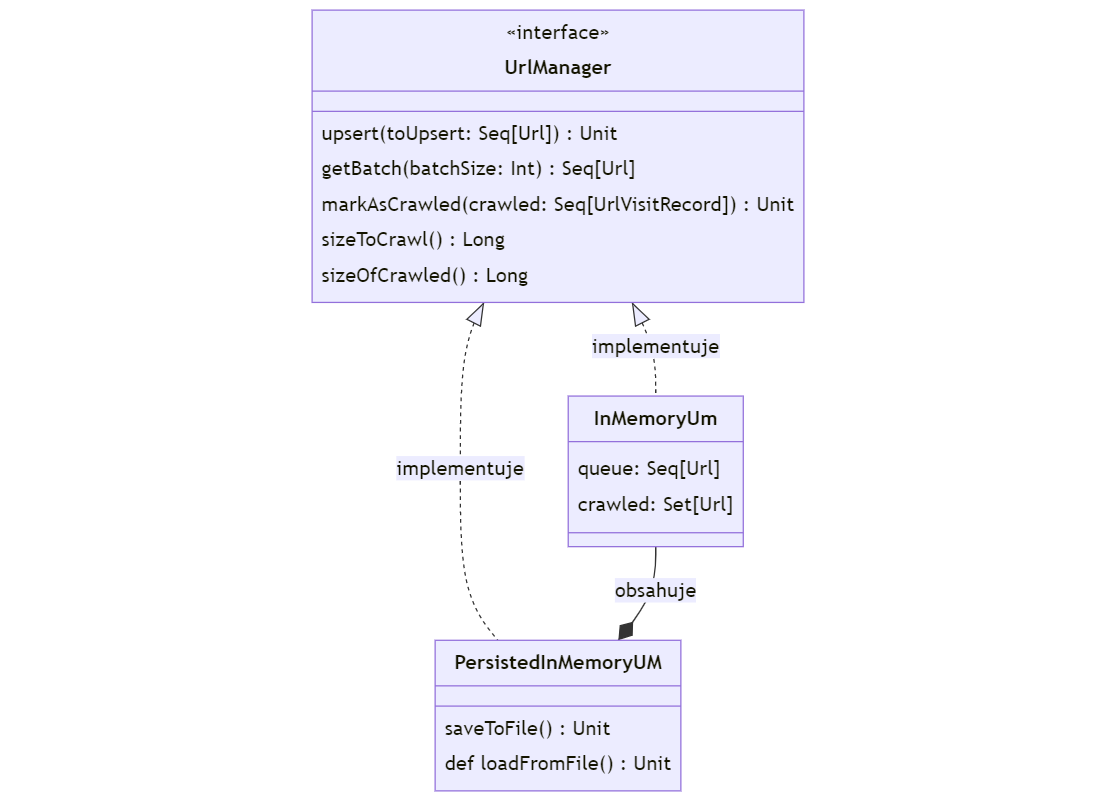
\includegraphics[width=1\textwidth]{figures/urlManagerChart.png}
    \caption{Diagram tried UrlManager\label{o:urlManChart}}
\end{figure}


\subsection{Repository}
Modul zodpovedný za ukladanie výsledkov. Vytvorené implementácie sú ukladanie do jedného CSV súboru, teda pridávanie výsledkov na jeho koniec. A ukladanie každého kroku do samostatného CSV súboru. Taktiež sme vytvorili implementáciu, ukladajúcu výsledky do pamäte. Tá je určenú len na testovanie zvyšných modulov. Jej rozhranie a implementácie sú znázornené na diagrame tried \ref{o:repoClassChart}. 

\begin{figure}[!ht]
    \centering
    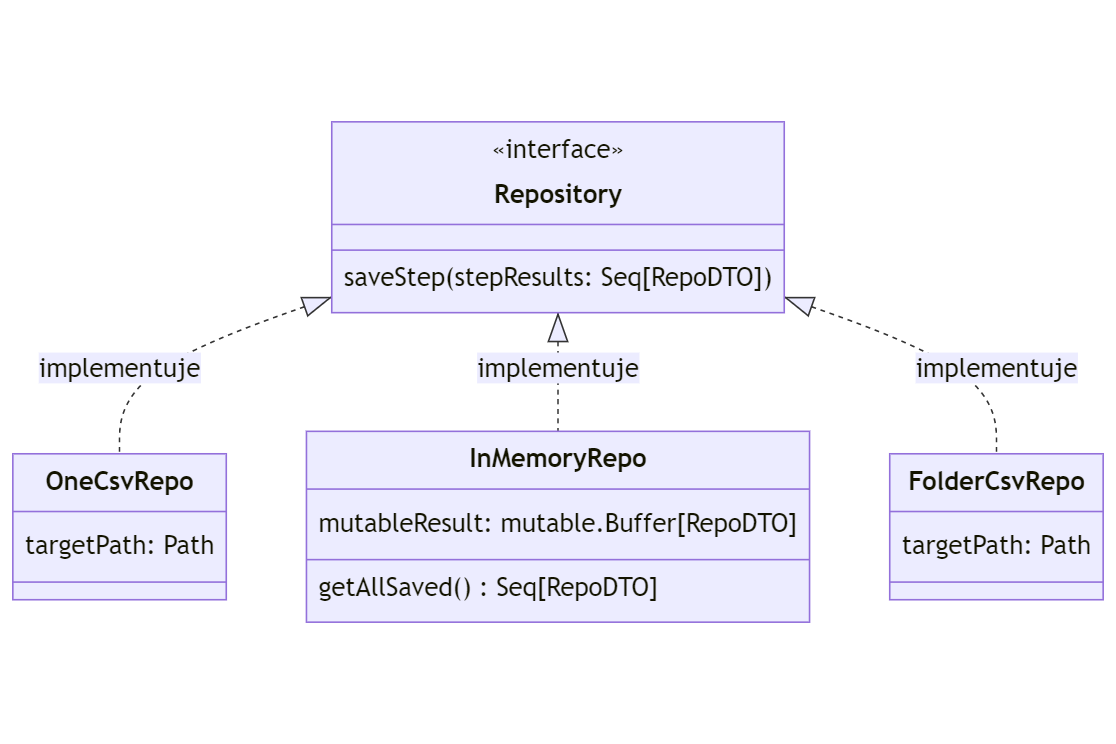
\includegraphics[width=1\textwidth]{figures/repositoryClassChart.png}
    \caption{Diagram tried Repository\label{o:repoClassChart}}
\end{figure}

\subsection{Modul crawlovania}
Nejde o samostatnú triedu ale o sadu funkcii, jedna volajúca druhú druhú. Je to jediné miesto paralelizácie a je striktne separované od zvyšku systému. Teda zvyšné moduly vôbec nevedia o paralelizácii a nemusia sa tomu prispôsobovať. Jeho úlohou je pre každú pridelenú adresu vrátiť CrawlResult. Na extrahovanie dát z HTML dokumentu a rozhodnutia či nájdená adresa je v prehľadávanej doméne využíva modul Extraktor.

\subsection{Extraktor}
V kóde je nazvaný DomainScraper. Slúži extrahovanie obsahu z HTML dokumentu a na určenie či adresa patrí pod jeho doménu. Každá implementácia je zameraná na jednu doménu. Pre pridanie novej domény na extrakciu je potrebné implementovať interface DomainScraper a pridať ho do zoznamu v objekte (scala alternatíva k java singletonu) SupportedDomains. Pre uľahčenie inicializácie crawlera navrhujeme v budúcnosti nastavovanie SupportedDomains cez CrawlerContext. Pre výber správneho extraktora pre spracovávanú adresú slúži DomainFilter s metódou getDomainScraper. Vzťahy medzi týmito triedami sú vyjadrené diagramom \ref{o:domScraperChart}.

\begin{figure}[!ht]
    \centering
    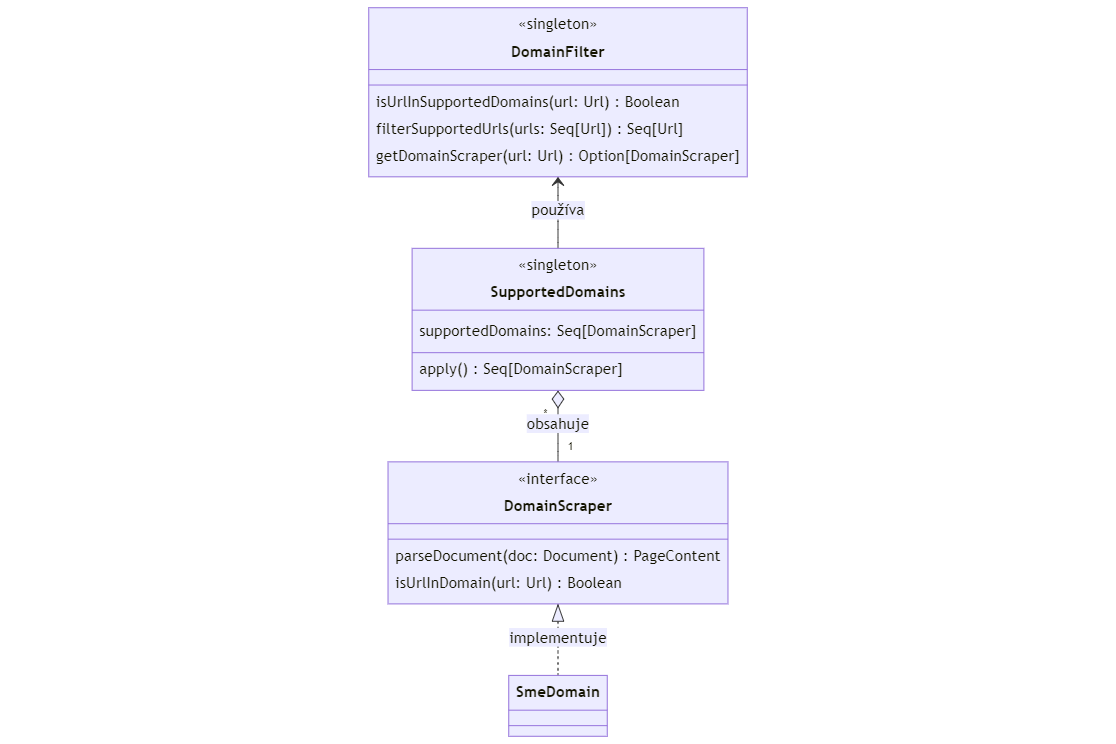
\includegraphics[width=1\textwidth]{figures/domainScraperChart.png}
    \caption{Diagram tried Extraktora\label{o:domScraperChart}}
\end{figure}

\subsection{Koordinátor}
Je to hlavná časť programu, sprostredkúvajúca komunikáciu medzi modulmi. V kóde je implementovaný ako trieda MyCrawler. 




\section{Pomocné triedy}
V programe používame triedy, ktoré nemôžeme považovať za samostatné moduly. V tejto podkapitole popíšeme stručne ich zodpovednosťa ich rozhranie voči zvyšku systému. 

\subsection{CrawlerContext}
Je to trieda slúžiaca na injektovanie závislostí crawleru. Teda aby sme mohli pri inicializácii crawlera určiť aké implementácie modulov chceme použiť a tým jednoducho meniť jeho správanie. Napríklad pri integračných testoch používať testovacie implementácie. Jeho štruktúru môžeme vidieť na diagrame tried \ref{o:classDiagramContextManual}.

\begin{figure}[!ht]
    \centering
    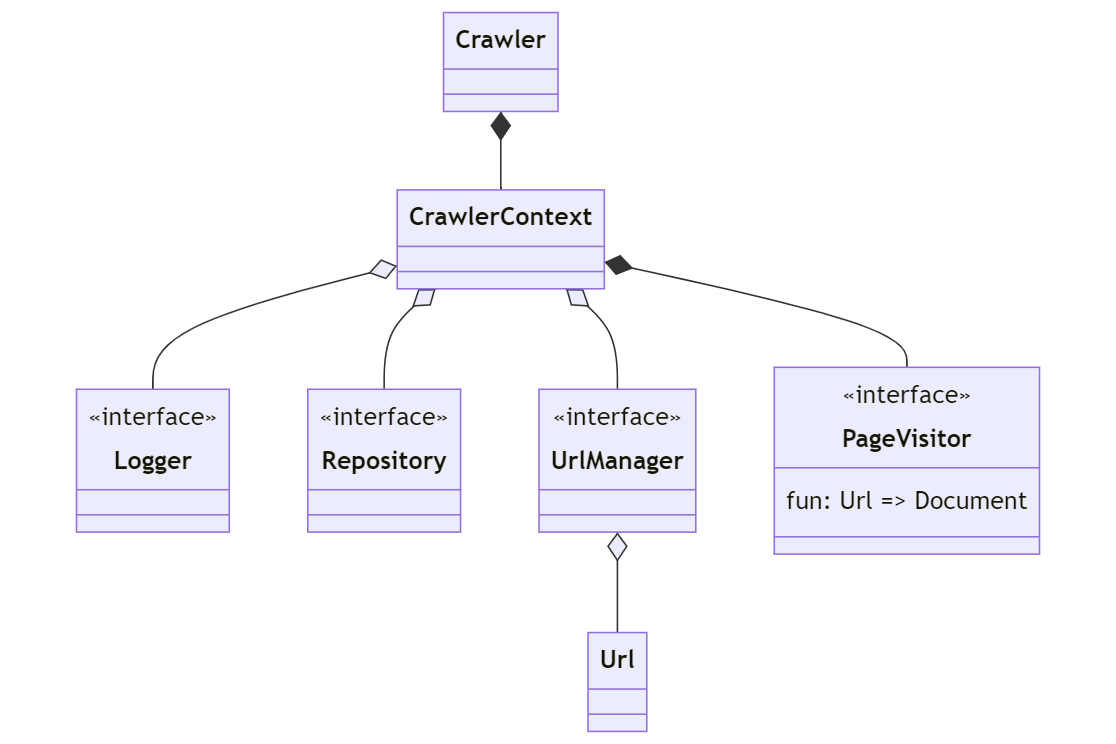
\includegraphics[width=1\textwidth]{figures/classDiagramContext.png}
    \caption{Diagram tried CrawlerContext\label{o:classDiagramContextManual}}
\end{figure}


\subsection{Logger}
Pomocný modul, slúžiaci na robenie záznamov o behu programu. Oproti bežnej implementácii umožňuje meranie trvania operácii. Napríklad ako dlho trvá zápis výsledkov. Takto vieme monitorovať priebeh crawlovania, čo je nápomocné pre jeho optimalizáciu a odhaľovanie chýb.



\section{Beh programu a paralelizácia}
Beh programu sme rozdelili do krokov. To nám umožnilo úplnú separáciu paralelného výpočtu od zvyšných modulov. Tým sme docielili, že iné moduly nemusia riešiť paralelizačnú logiku. Jeden krok je vyjadrený pomocou sekvenčného diagramu \ref{o:seqStepManual}.

\begin{figure}[!ht]
    \centering
    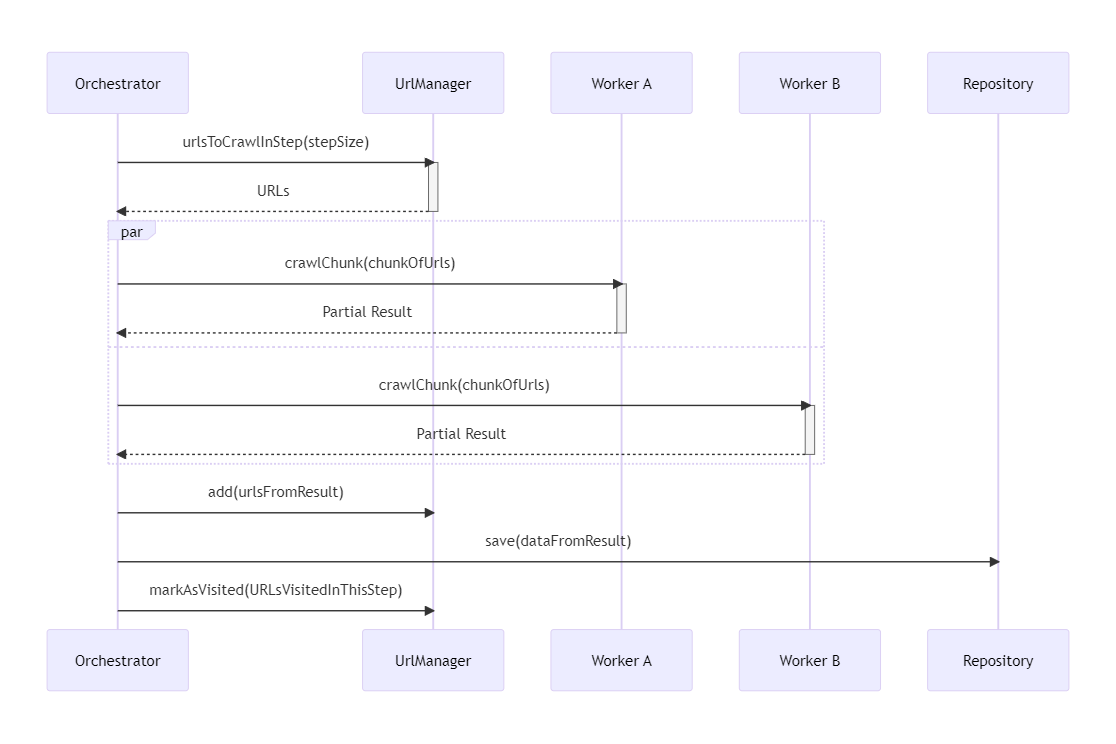
\includegraphics[width=1\textwidth]{figures/seqDiagCrawlStep.png}
    \caption{Sekvenčný diagram jedného kroku\label{o:seqStepManual}}
\end{figure}



% zivotopis autora
%\curriculumvitae\protect
%Táto časť\/ je nepovinná. Autor tu môže uviesť\/ svoje biografické
%údaje, údaje o~záujmoch, účasti na~projektoch, účasti na~súťažiach,
%získané ocenenia, zahraničné pobyty na~praxi, domácu prax, publikácie
%a~pod.
\end{document}
